\chapter{Results}\label{sec:Results}

During the course of this project, an autonomous mobile robot capable of preforming warehouse pick and place tasks has been set up. Necessary mechanical modifications has been done to the UGV platform in order to accommodate extra sensors and a robotic manipulator. Then, sensors and algorithms has been configured to build a demonstration of how this system could be used to preform a warehouse automation task. Testing has first been done separately on both the the autonomous navigation system and the pick and place system. Then, the entire warehouse automation pipeline has been deployed and tested through the Husky Master Node.

 % \section{Hardware}\label{R:Hardware}
 % As hardware aspects and some hardware design has been discussed in section \ref{sec:M:ConceptualDesign} \ref{sec:H:Hardware}, it is natural to include the result of the design process.

% \subsection{General Arrangement} \label{sec:R:GeneralArrangement}
% Looking at figure \ref{fig:huskyComplete}, there is a radar mounting bracket with two Texas Instrument radars at the front of the Husky A200 UGV. This radar array is a part of another Master's Thesis by Didrik Robsrud running in parallel to this project. It is therefore not a part of the general arrangement drawing (figure \ref{fig:general_arrangement}) in section \ref{M:H:GeneralArrangement}. Apart from this radar array, the auxiliary components on the UGV is mounted in accordance to the general arrangement. All components are powered  through the Husky A200's power supply in accordance with the electrical interface drawing (figure \ref{fig:circuit_diagram}) in section \ref{M:H:ElectricalInterface}.



% \subsection{Accessory Mounting Frame}\label{sec:R:H:AccessoryMountingFrame}
% As mentioned in section \ref{sec:M:H:AccessoryMountingFrame}, an accessory mounting frame was made to accommodate auxiliary sensors and equipment. The frame is made out of $20X20[mm]$ aluminium strut profiles \cite{boshRexrothAluminium}, cut to length and put together according to the design in section \ref{sec:M:H:AccessoryMountingFrame}. \ref{sec:M:H:ANH:LidarAndCameraMount}, was fixed to the top of the accessory frame along with the OS1 LiDAR one camera. The complete physical UGV with the it's accessory frame including the LiDAR mount can be seen in figure \ref{fig:huskyComplete}.


% \subsection{Manipulator} \label{sec:R:H:Manipulator}
% The Interbotix VX300 manipulator, described in section \ref{sec:M:H:P&PH:Manipulator}, is mounted to the Husky A200 UGV in accordance with the description. An extra aluminium strut was added at the rear of the UGV to create extra mounting points for the manipulator. It can be seen how the manipulator is mounted on the husky in figure \ref{fig:M:H:CHS:CadHuskyComplete}. 

% \subsection{Manipulator Mounted Camera}\label{R:H:ManipulatorMountedCamera}
% As described in section \ref{sec:M:H:P&PH:ManipulatorMountedCamera}, a manipulator mounted camera has been set up. Section \ref{sec:M:H:P&PH:ManipulatorMountedCamera} also describes how this camera is mounted on the manipulator with a bracket designed for the task. The resulting configuration can be seen in figure \ref{fig:R:H:M:M:MMC:Vx300Complete}.



\section{Digital Twin} \label{sec:R:DigitalTwin}
The complete configuration is set up with ROS2 so that a digital twin is possible to visualise in Rviz2. Compatibility with ROS2 allows for example visualisation of the robot on top of a 2D map while autonomously navigating through the environment. Figure \ref{fig:R:H:DT:DigitalTwin} shows the digital twin visualised in Rviz2.

\begin{figure}[H]
  \centering
  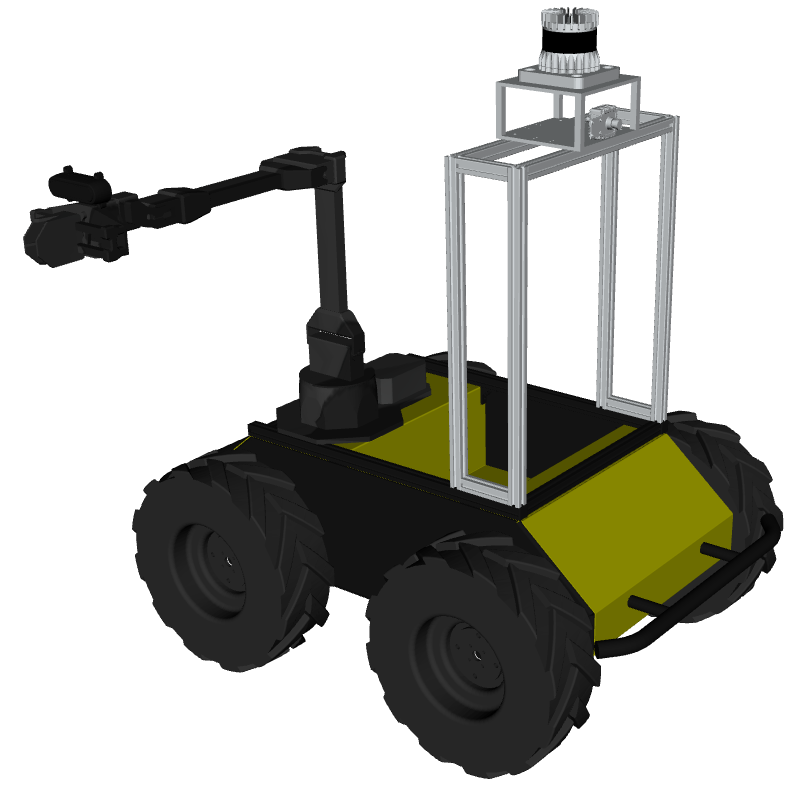
\includegraphics[width = 0.6\textwidth]{Figures/figDigitalTwin.png}
  \caption{Rviz2 visualisation of complete setup running in ROS2. This acts as a digital twin corresponding to the physical robot.}
  \label{fig:R:H:DT:DigitalTwin}
\end{figure}

\section{Autonomous Navigation} \label{sec:R:AutonomousNavigaion}
% The autonomous navigation is set up in ROS2 according to the descriptions in the method. In the context of this thesis, the UGV is a part of the autonomously navigating platform. Therefore the resulting configuration of the UGV will be described here. This section will present results regarding the autonomously navigating platform, starting with SLAM and then autonomous navigation results. All testing was preformed at UiA Campus Grimstad.

\subsection{Simultaneous Localisation and Mapping}\label{sec:R:AN:SLAM}
Testing of SLAM was done by running the complete UGV setup with SLAM and autonomous navigation. The SLAM algorithm would gen  map while travelling from the machine lab at campus to the elevators, this is a distance of about \textbf{DISTANCE}, and an area of about \textbf{AREA}. The resulting map can be seen in figure \ref{fig:R:AN:SLAM:figUiaMap}.

\begin{figure}[H]
  \centering
  \includesvg[angle=90, width = 0.5\textwidth]{Figures/figUiaMap.svg}
  \caption{Map of Machine Lab and Corridor at UiA Campus Grimstad. The map has been generated through SLAM with an autonomous mobile robot.}
  \label{fig:R:AN:SLAM:figUiaMap}
\end{figure}

\subsection{Navigation}\label{sec:R:AN:Navigation}
Navigation was tested by running the complete setup, together with SLAM, as mentioned in section \ref{sec:R:AN:SLAM}. As the map was generated on-the go, goal poses were manually updated by the operator as the map continued to be updated. Figure \ref{fig:R:H:SLAM:figNavUia} how the autonomous navigation is visualised on the operators computer using Rviz2.

\begin{figure}[H]
  \centering
  \begin{minipage}[b]{0.49\textwidth}
        \centering
        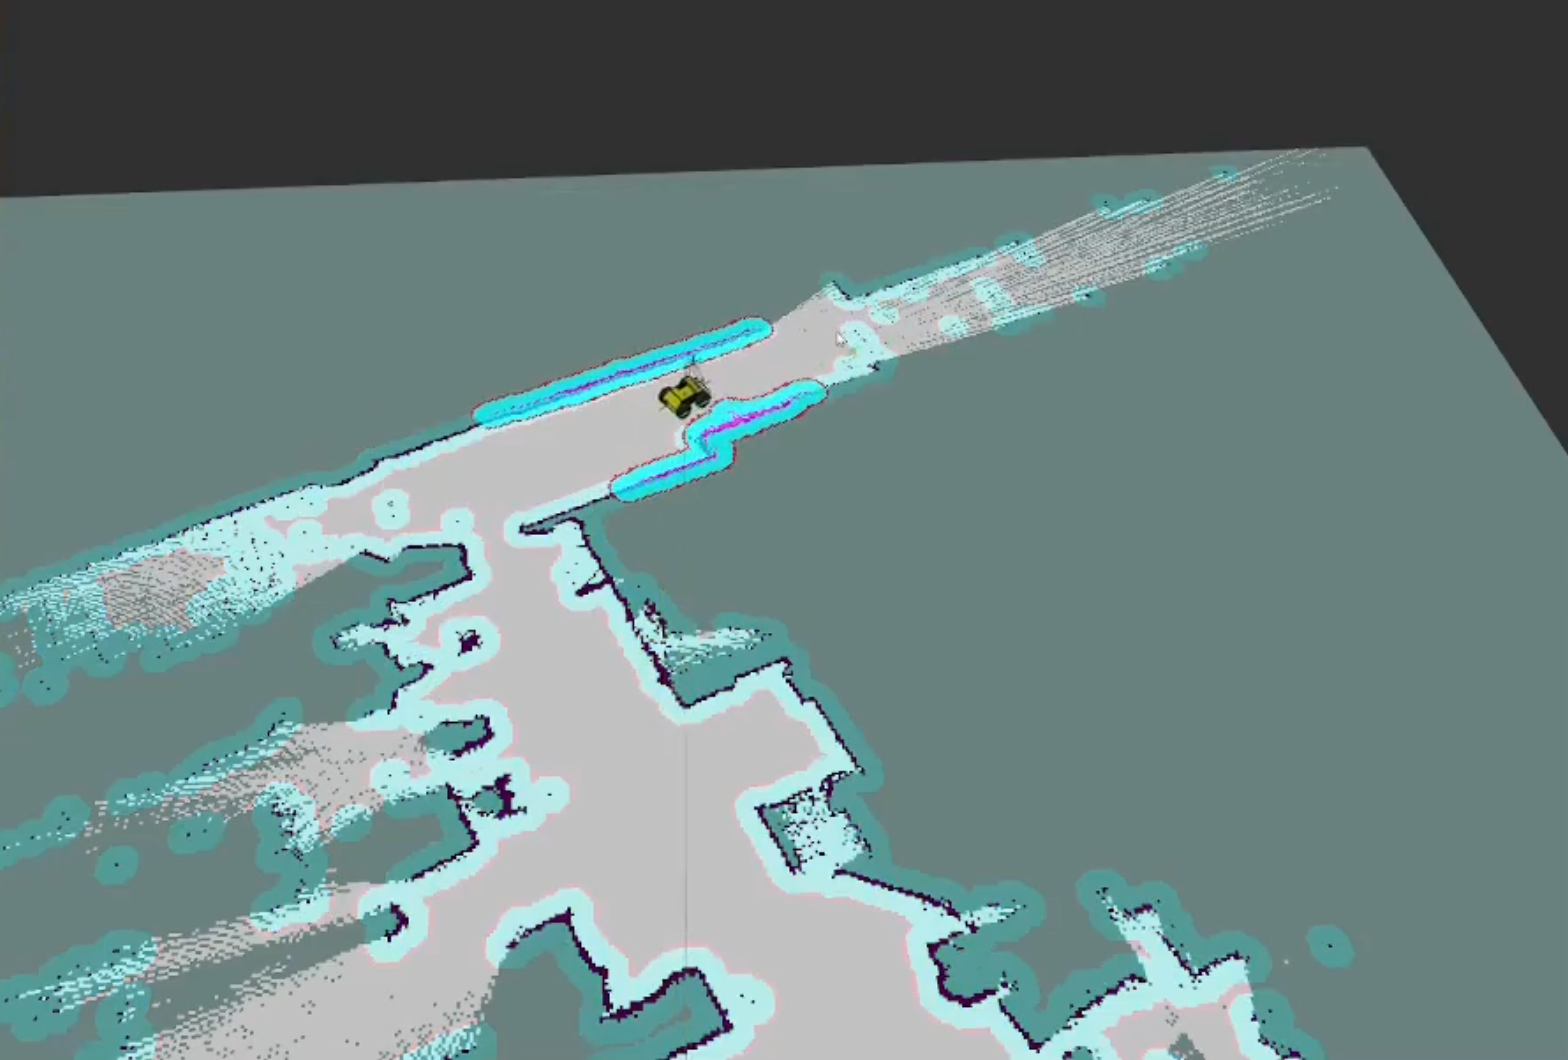
\includegraphics[width = 0.9\textwidth]{Figures/figNavUia2.png}
  \end{minipage}
  \hfill
  \begin{minipage}[b]{0.49\textwidth}
    \centering
    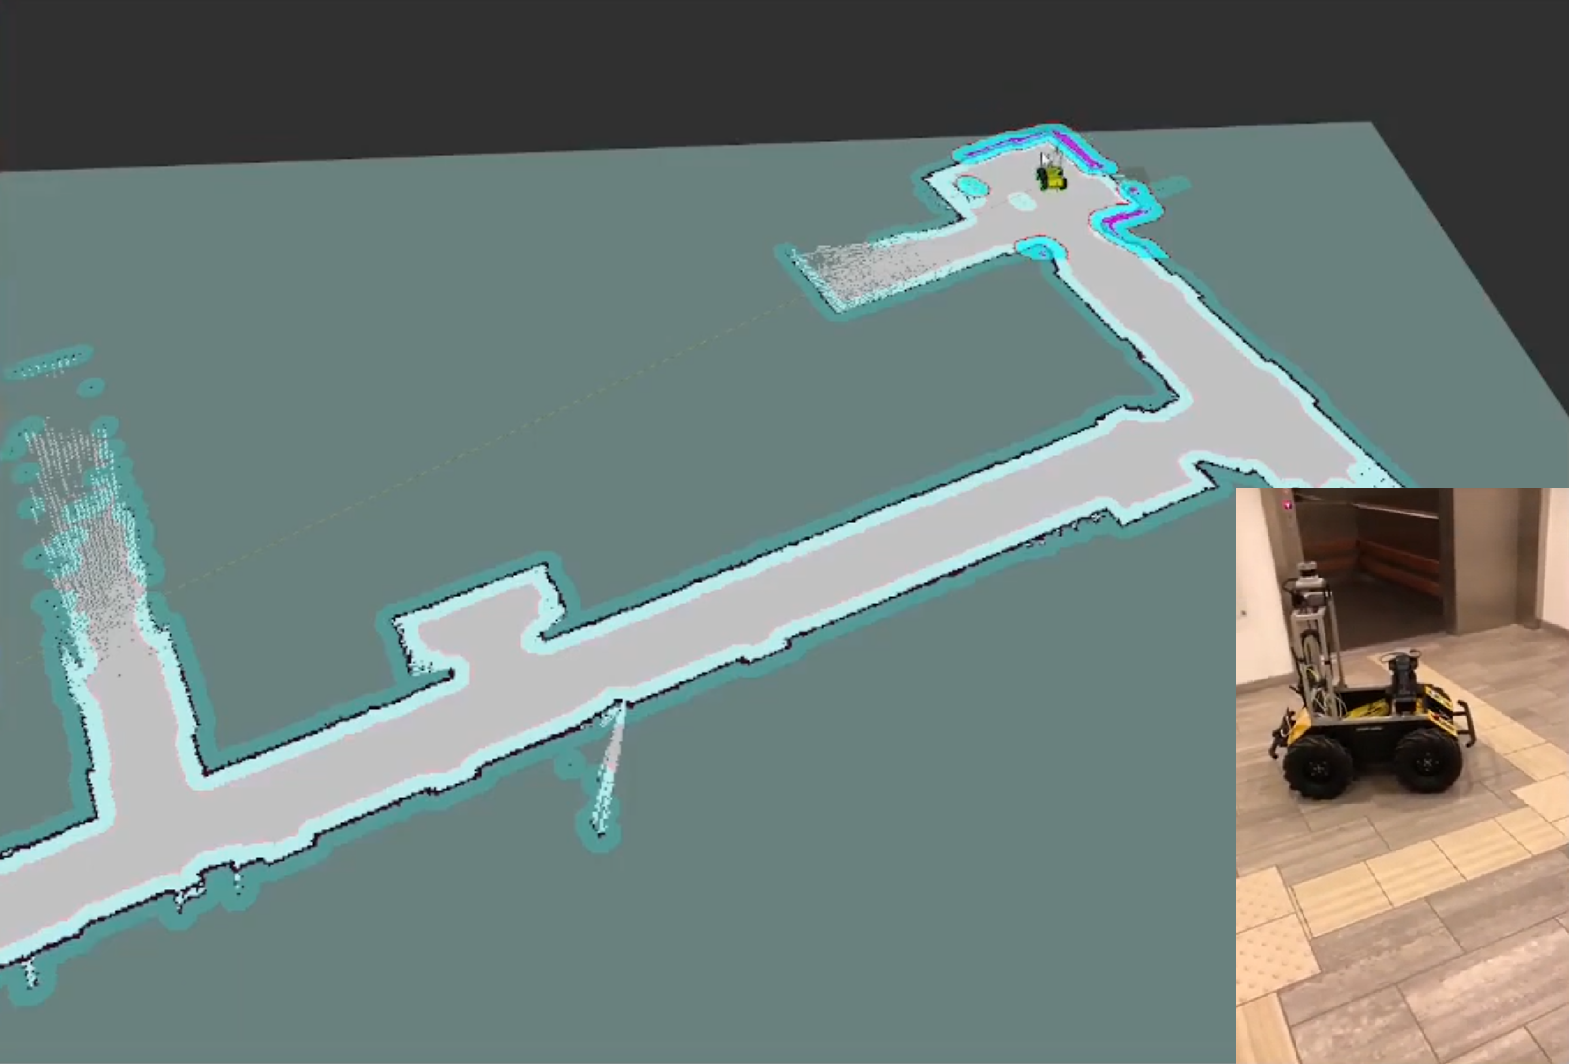
\includegraphics[width = 0.9\textwidth]{Figures/figNavUia4.png}
  \end{minipage}
  \caption{Mobile robot Running NAV2 along with SLAM on ROS2. This is a visualisation of Rviz2 where the mobile robot is illustrated as a 3D model on top of the generated map.}
  \label{fig:R:H:SLAM:figNavUia}
\end{figure}


\subsubsection{Collision Avoidance}
During navigation testing, collision avoidance was tested by placing a person in front of the robot. Figure \ref{fig:R:AN:N:CA:CollisionAvoidance1} and \ref{fig:R:AN:N:CA:collisionAvoidance2} is taken from the Rviz2 visualisation of the navigation system, showing this test. In figure \ref{fig:R:AN:N:CA:CollisionAvoidance1} the robot is moving without anything in it's way. A few moments later, a pedestrian has moved in front of the robot. The resulting trajectory can be seen as the green line in figure \ref{fig:R:AN:N:CA:collisionAvoidance2}.

\begin{figure}[H]
  \centering
  \begin{minipage}[b]{0.49\textwidth}
        \centering
        \includegraphics[width = 0.9\textwidth]{Figures/figuiaCollisionAvoid3.png}
        \caption{Robot navigating through a hallway. After this, a pedestrian will move in front of the robot and be detected by the local cost-map. Notice how the trajectory (green line) goes straight towards the goal.}
        \label{fig:R:AN:N:CA:CollisionAvoidance1}
  \end{minipage}
  \hfill
  \begin{minipage}[b]{0.49\textwidth}
    \centering
    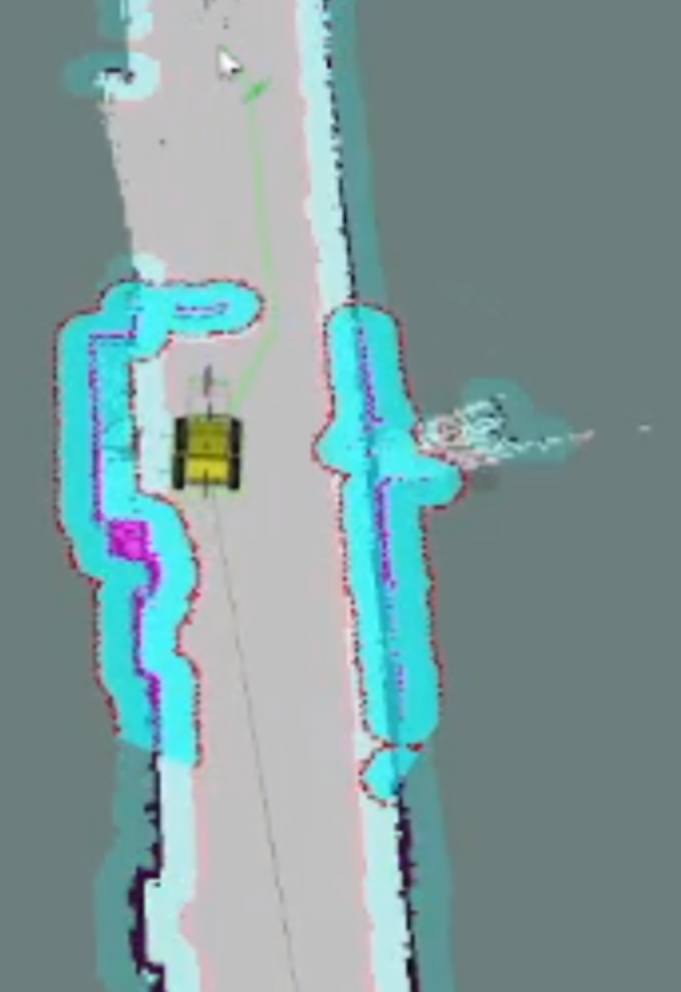
\includegraphics[width = 0.86\textwidth]{Figures/figUiaCollisionAvoid4.png}
    \caption{Robot navigating around obstacle. In this figure, a pedestrian is standing in the way of the robot. Notice how the trajectory (green line) goes around the object.}
    \label{fig:R:AN:N:CA:collisionAvoidance2}
  \end{minipage}
\end{figure}

\section{Pick and Place} \label{R:PickAndPlace}
% Pick and place operations is achieved through a combination of three systems. The first system is the VX300 manipulator itself and it's ROS2 Moveit2 packages described in section \ref{sec:M:MRC:Manipulator}. The second system is the machine vision system described in section \ref{sec:M:MRC:MachineVision}. This includes the vision camera, its drivers and the AprilTag based object detection system. The last system needed is the custom pick and place ROS2 package described in section \ref{sec:M:A:HuskyPickAndPlace}. Results regarding object detection and the custom pick and place ROS2 package will be presented.



% \subsection{Custom ROS2 Packages}
% The custom ROS2 packages has been built and tested around a specific robotic system. It is not likely that it will work for other types of robotic systems out of the box. 

\subsubsection{Custom Scene Publisher Package}
As mentioned in section \ref{sec:M:PAP:SceneGeometryPublisher}, a custom ROS2 package was made to publish collision boxes to the planning scene. The package is run automatically when launching the manipulator using the custom launch file \lstinline{xavier2_launch.py} from the git repository made for this projects manipulator\cite{husky_vx300_repo}. The result is given in figure \ref{fig:R:P&P:CSP:scenePublisher1} and  \ref{fig:R:P&P:CSP:scenePublisher2} where the manipulator has first been initiated in an empty space in figure \ref{fig:R:P&P:CSP:scenePublisher1}, then the package has been launched and the collision boxes that encapsulate the robot has been published in figure \ref{fig:R:P&P:CSP:scenePublisher2}. These collision boxes are usually hidden in Rviz2 in favour of nicer visuals shown in section \ref{sec:R:DigitalTwin}.

\begin{figure}[H]
  \centering
  \begin{minipage}[b]{0.49\textwidth}
        \centering
        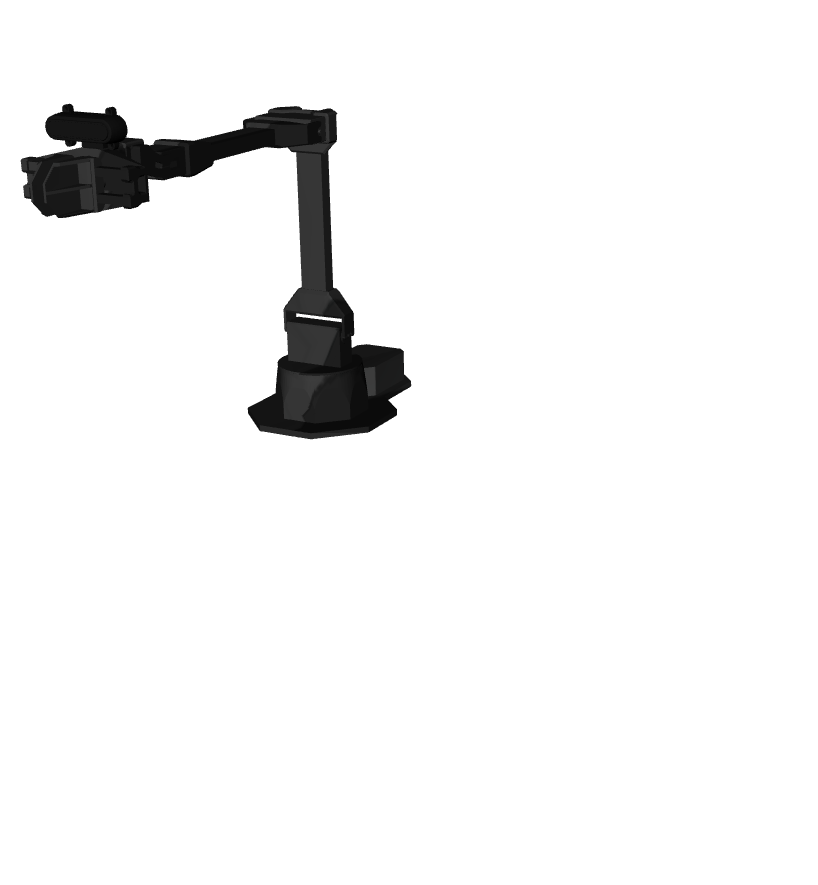
\includegraphics[width = 0.9\textwidth]{Figures/figScenePublisher1.png}
        \caption{Manipulator initiated with Moveit2 and visualised in Rviz2.}
        \label{fig:R:P&P:CSP:scenePublisher1}
  \end{minipage}
  \hfill
  \begin{minipage}[b]{0.49\textwidth}
    \centering
    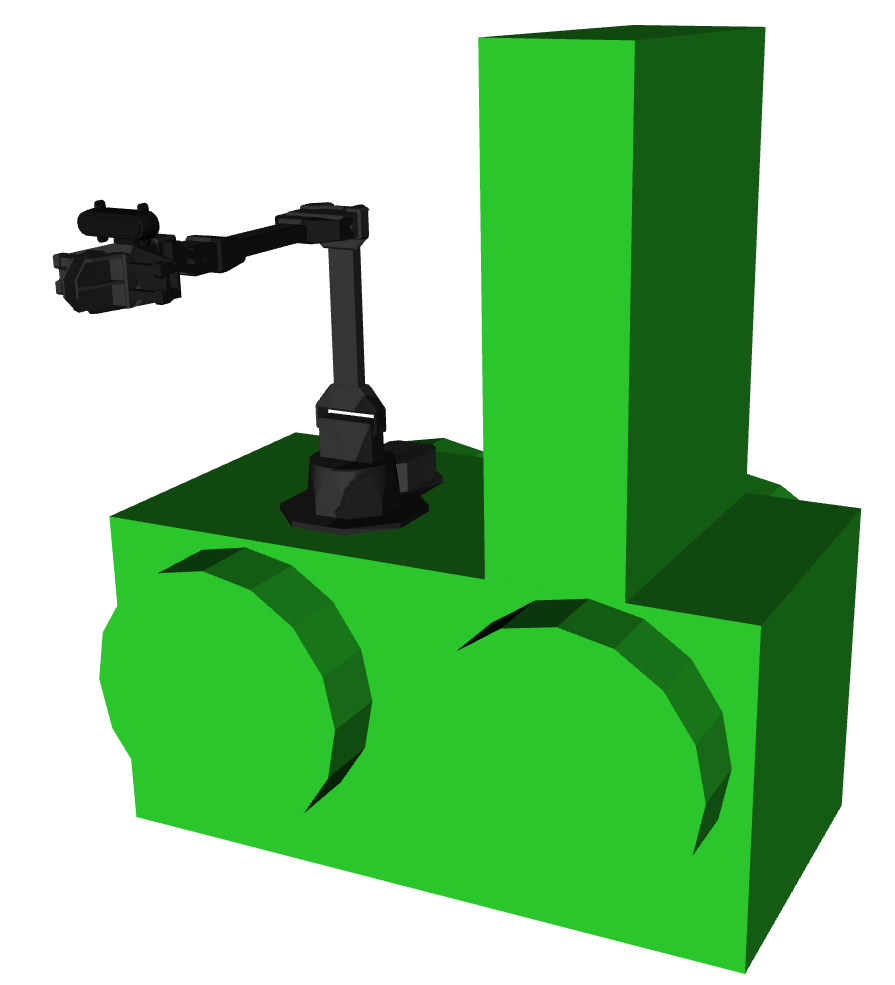
\includegraphics[width = 0.86\textwidth]{Figures/figScenePublisher2.png}
    \caption{Manipulator initiated with Moveit2 and visualised in Rviz2. Collision boxes are published to the planning scene using the custom Scene Publisher ROS2 package.}
    \label{fig:R:P&P:CSP:scenePublisher2}
  \end{minipage}
\end{figure}


\subsubsection{Husky Pick and Place Package}
A custom ROS2 package has been made to enable control of the manipulator and get feedback about current operation through the ROS2 network's topic system. The design of this package is described in section \ref{sec:M:A:HuskyPickAndPlace}. Testing has been done to tune the robot's move sequences and to verify the robustness of the ROS2 topic based command and feedback system. 

\textbf{Do some testing and write a bit about it here}

\section{Top Level}
% The full warehouse automation pipeline is set up using the custom ROS2 package "Husky Master Node" described in section \ref{sec:M:A:HuskyMasterNode}. Running this node results in the UGV autonomously navigating to a predefined pick location before running the pick operation. The pick operation includes using machine vision to detect and estimate the pose of the object before picking. After picking, the UGV moves to the place location and the place operation is preformed. Finally, the UGV will return to it's starting position. The complete operation where the robot moves to a pick location, picks an object using MV, moves to a place location, places the object and moves back home was performed twice in a row with success.

Testing of the complete warehouse automation pipeline has been preformed in the machine lab at UiA Campus Grimstad. Prior to launching the "Husky Master Node", the complete autonomous navigation system including SLAM has been brought up and is ready to take commands. The pick and place system, is also brought up an ready to take commands. This includes the AprilTag machine vision system.

Figure \ref{fig:R:WA:finalExperiment1} illustrates initiation of the Husky Master node and navigation to the first goal. This is the "pick pose".

\begin{figure}[H]
  \centering
  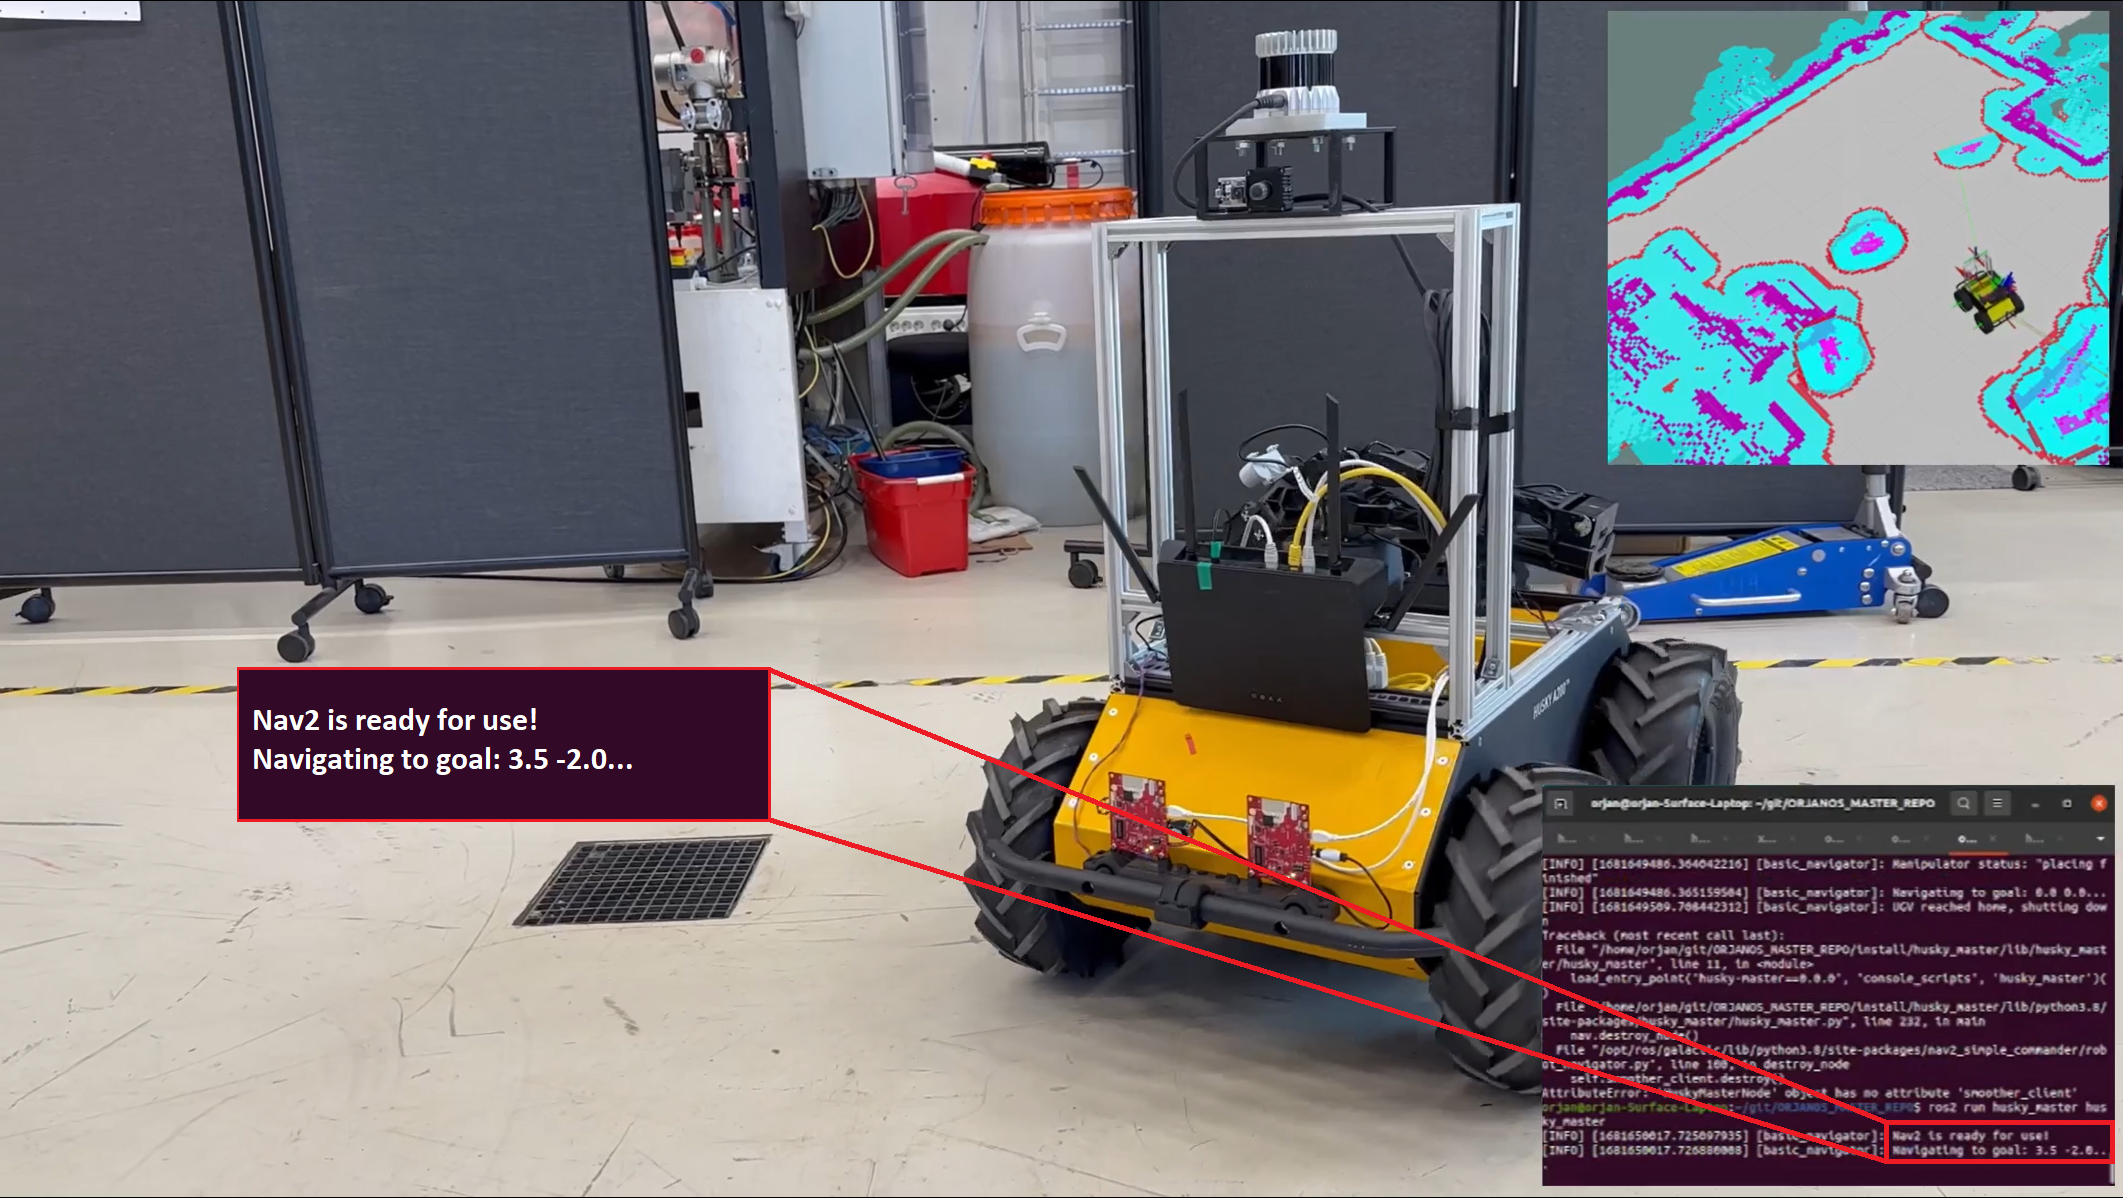
\includegraphics[width = 0.8\textwidth]{Figures/figHuskyFinalExperiment1.png}
  \caption{This figure illustrates initiation of Husky Master Node and navigation towards the first goal during testing. The map in the top right corner corresponds to the actual position of the mobile robot. The terminal window in the lower right corner provides some info about the progress in the warehouse automation pipeline.}
  \label{fig:R:WA:finalExperiment1}
\end{figure}

Figure \ref{fig:R:WA:finalExperiment2} illustrates the picking operation during the warehouse automation task. The mobile robot has reached it's picking pose and is currently performing a picking operation. Interactions between the Husky Master Node and the Pick and Place Node can be seen in the bloated section of the terminal window. The instance figure \ref{fig:R:WA:finalExperiment2} is taken, the manipulator has detected the object, and then placed it's end-effector directly above the object for the machine vision system to get more accurate measurements before picking the object.

\begin{figure}[H]
  \centering
  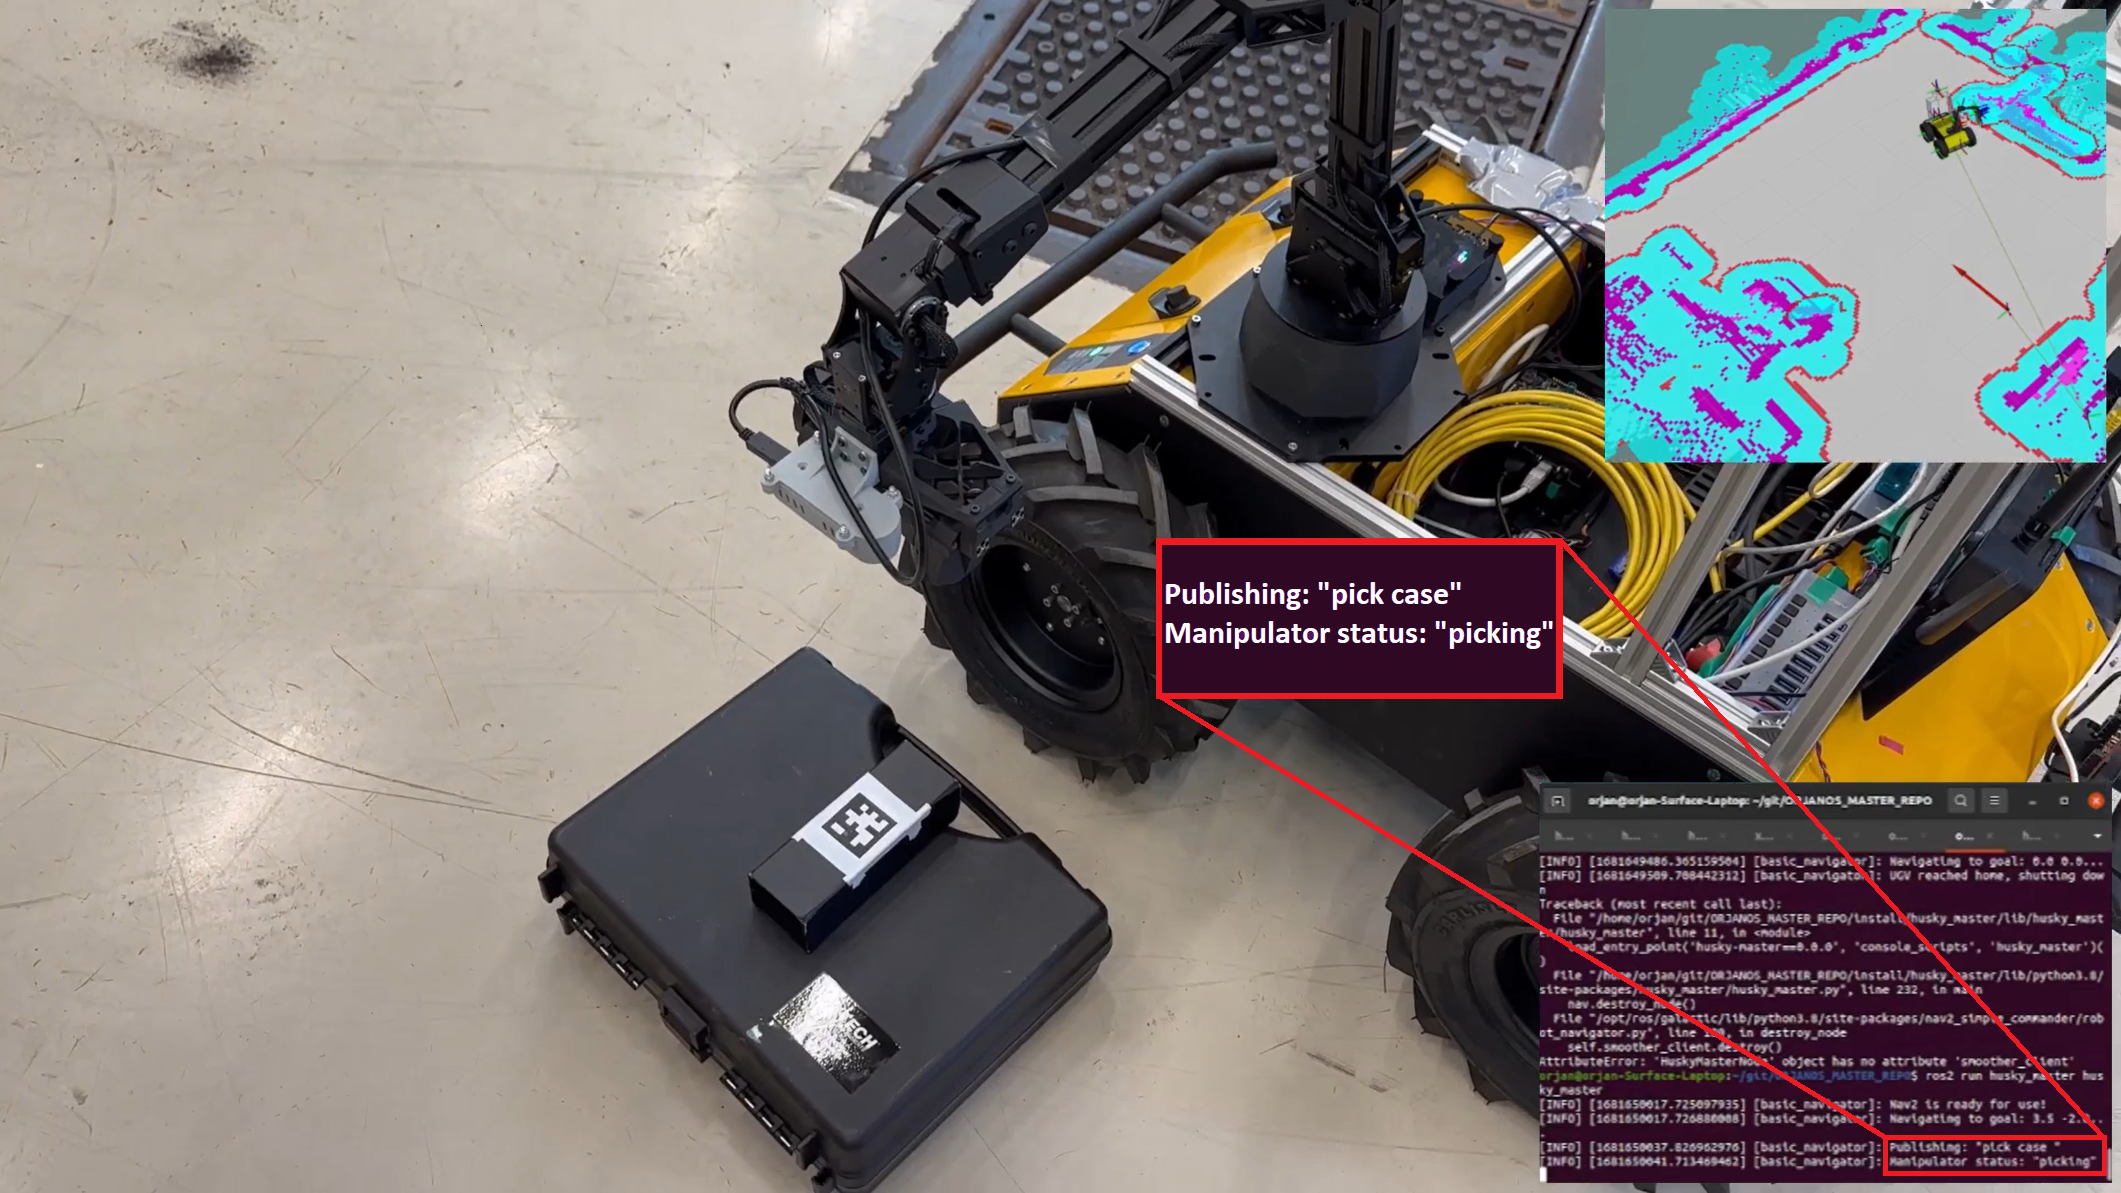
\includegraphics[width = 0.8\textwidth]{Figures/figHuskyFinalExperiment2.png}
  \caption{This figure illustrates picking operation during the warehouse automation task. In this instance, the manipulator has positioned itself directly above the object to give a more accurate measurement before picking. Relevant command and feedback between the Husky Master node and Pick and Place node can be seen in the bloated section from the terminal.}
  \label{fig:R:WA:finalExperiment2}
\end{figure}

% \begin{figure}[H]
%   \centering
%   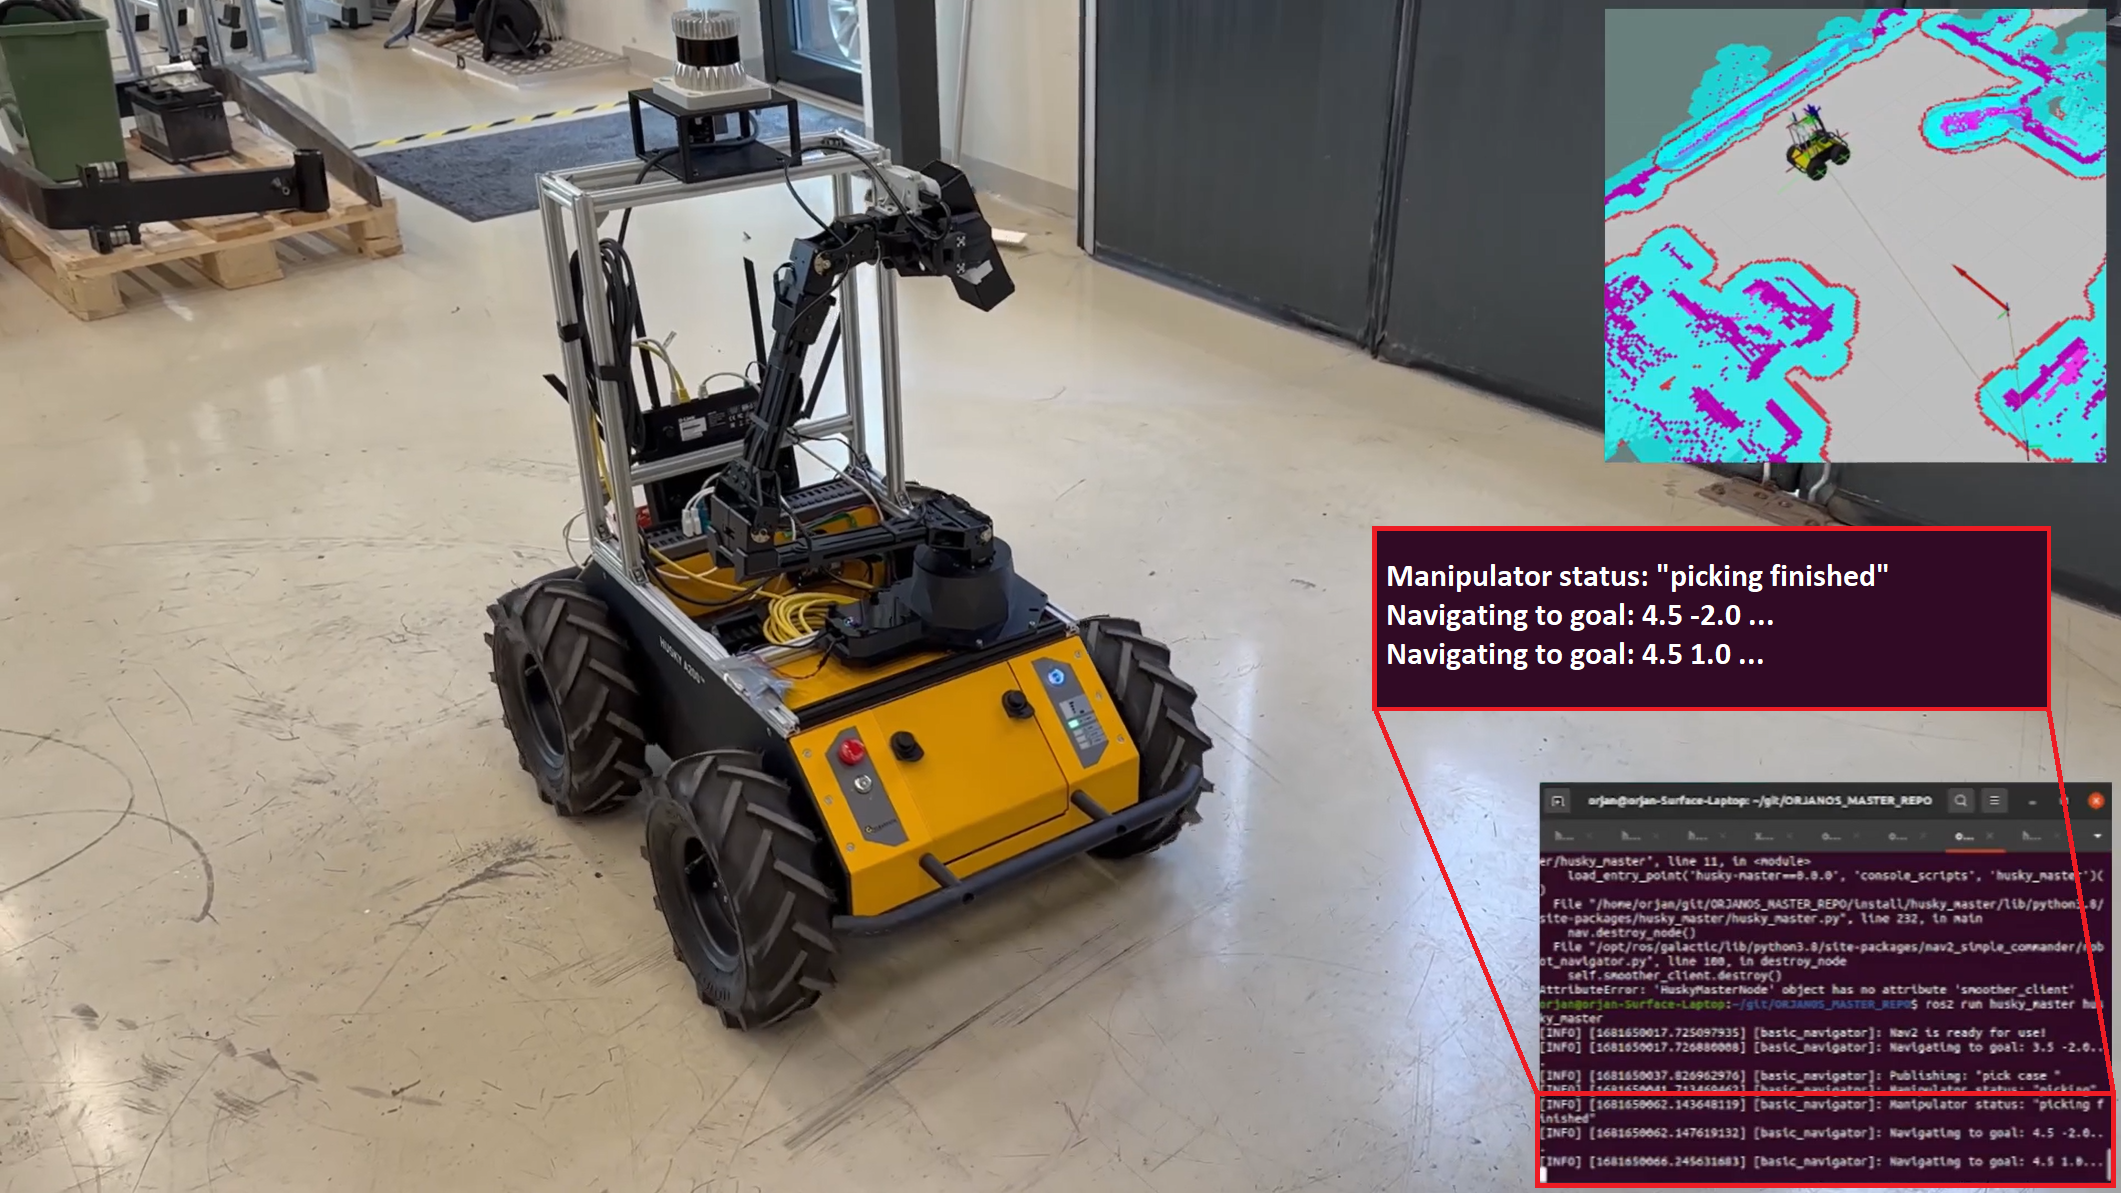
\includegraphics[width = 0.8\textwidth]{Figures/figHuskyFinalExperiment3.png}
%   \caption{This figure illustrates }
%   \label{fig:R:WA:finalExperiment3}
% \end{figure}

The placing operation of the warehouse automation task is shown in figure \ref{fig:R:WA:finalExperiment4}. As with figure \ref{fig:R:WA:finalExperiment2}, interactions between the Husky Master Node and the Pick and Place Node can be seen in the bloated terminal section. The object has been dropped to the floor moments before figure \ref{fig:R:WA:finalExperiment4} is captured.

\begin{figure}[H]
  \centering
  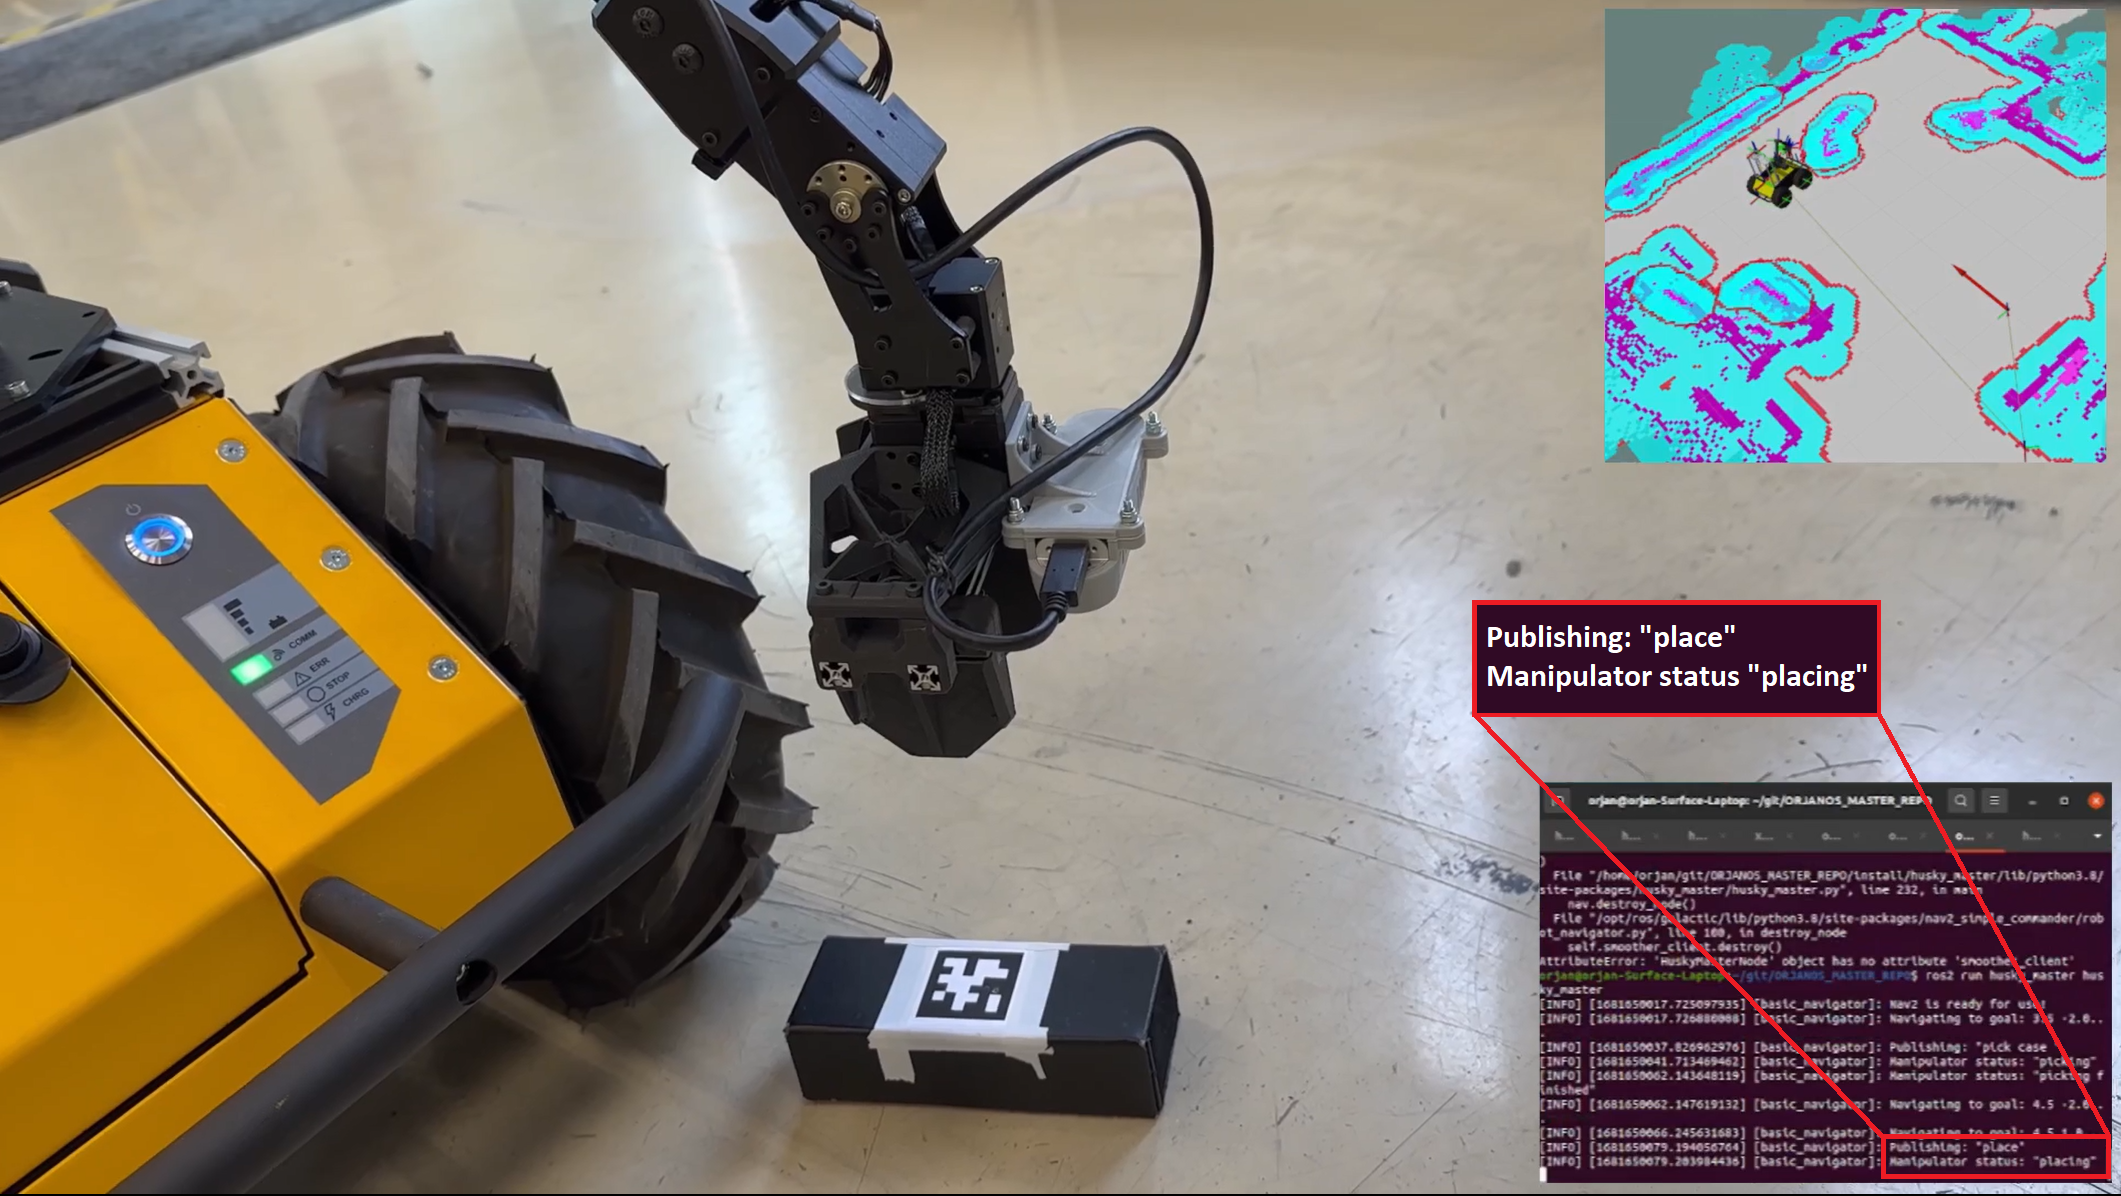
\includegraphics[width = 0.8\textwidth]{Figures/figHuskyFinalExperiment4.png}
  \caption{This figure illustrates the placing operation during the warehouse automation task. Notice from the map in the top left corner that the mobile robot has moved to a different location. Relevant command and feedback between the Husky Master node and Pick and Place node can be seen in the bloated terminal.}
  \label{fig:R:WA:finalExperiment4}
\end{figure}

After placing is finished, the mobile should return to it's starting position. This is illustrated in figure \ref{fig:R:WA:finalExperiment5}. There is a red arrow pointing at a coordinate frame in figure \ref{fig:R:WA:finalExperiment5}. This is the last known coordinate of the placed object. The bloated terminal section indicates that the placing operation is finished and that the robot is moving to "0.0 0.0 ...", in other words, start position.

\begin{figure}[H]
  \centering
  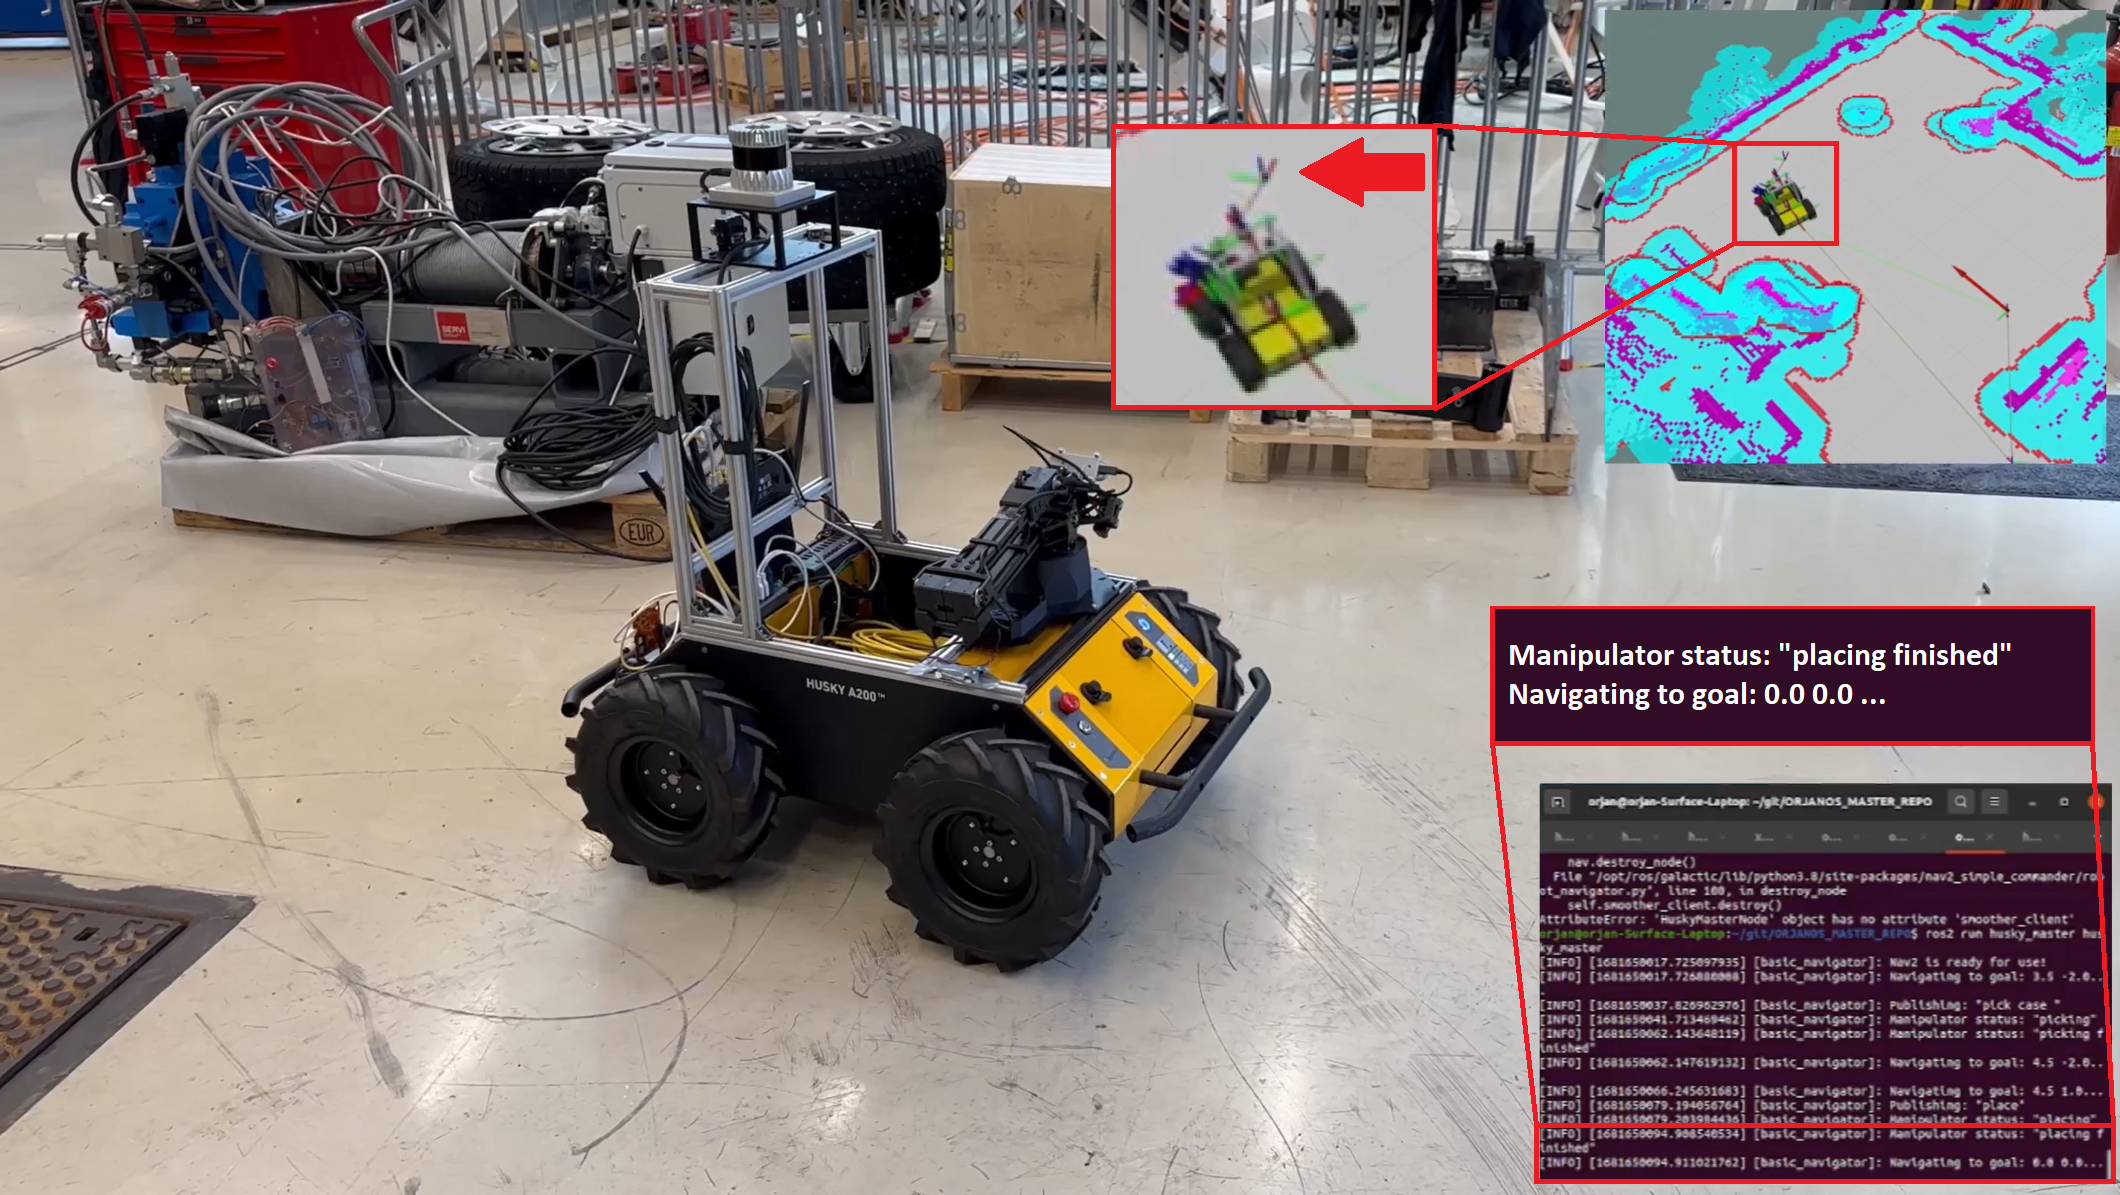
\includegraphics[width = 0.8\textwidth]{Figures/figHuskyFinalExperiment5.png}
  \caption{This figure illustrates that the mobile robot is navigating back to it's starting pose after placing the object. The bloated section from the map has a red arrow pointing at a coordinate frame behind the mobile robot. This is the last known coordinate of the placed object.}
  \label{fig:R:WA:finalExperiment5}
\end{figure}









%aj \section{experiment}
% write about different environment where experiment is done

% \subsection{indoor environment}

% \subsection{ware house environment}

% \section{Results}
% write that algorithms in ch 3.. was implemented to get the results with accuracy and precision, error ...

% KPI for each of functionality - show that it could navigate without collision, localize and estimate the pose of object with error xxx, pick it and place it at predefined location with error xxx

% \section{Pick and Place}



% \section{Autonomous Navigation}
% Bad kinematic design on Husky

% \section{Tag Detection}
% Worked like a charm

% \section{Pick and Place}
% Small and weak manipulator

% \section{Husky Master}
%  Unpolished Algorithm

%  \section{Husky Pick and Place}
%  Unpolished algorithm
%  Not general
%  not ideal launch file
 
%  Two methods for picking were discussed. Both of these places restrictions on the pose/shape of the objects t be picked. One method of picking bases itself on picking the objects from the side. That is, the manipulator moves in from the side of the object when gripping it. This 

%  \section{Scene Geometry Publisher}
%  Not ideal launch file
%  General design, but not general launch

 %Conclusion and Discussion